\chapter{Analytical Forces Induced by Dislocations on Linear Rectangular Surface Elements}
\label{c:lin_rect}
	%
	\section{Forces Exerted by a Dislocation Line Segment on Linear Rectangular Surface Elements}
	\label{s:f_lin_rect}
		%
		Coupling \kwd{ddd} to \kwd{fem} requires the traction field $ \tns{\sigma^{\infty}}(\vec{x}) \cdot \vec{n}(\vec{x}) $ to be distributed among the set of relevant discrete nodes of a \kwd{fe} or \kwd{be} model. This is usually achieved as follows,
		\begin{align}\label{e:ddd_fem_force}
			\vec{F}^{(m)} = \int_{S^{e}} \left[\tns{\sigma^{\infty}}(\vec{x}) \cdot \vec{n}(\vec{x})\right] N_{m}(\vec{x})\; \rvar{d}S_{e}\,,
		\end{align}
		where $ \rvar{d}S_{e} $ is the infinitesimal surface element with surface area $ S_{e} $. $ N_{m}(\vec{x}) $ are so-called shape functions (interpolation functions) that distribute  the traction field among the surface element's nodes.
		
		The problematic singularity associated with the classical Volterra dislocation is avoided by using the non-singular formulation of \citet{a_non-singular_continuum_theory_of_dislocations}. The stress field of a dislocation in a homogenous infinite linear elastic domain can be calculated as a contour integral along the loop \cite{mura_t},
		\begin{align}\label{e:field_stress}
			\sigma_{ij}^{\infty}(\vec{x}) = C_{ijkl} \oint \epsilon_{lnh} C_{pqmn} \dfrac{\partial G_{kp}(\vec{x} - \vec{x'})}{\partial x_{q}} b_{m} \rvar{d}x'_{h}\,,
		\end{align}
		where $ C_{ijkl} $ is the elastic stiffness matrix, $ \epsilon_{lnh} $ the permutation operator, \kwds{bv} the \kwd{bv}, $ \vec{x'} $ the coordinate that spans the dislocation, and $ G_{kp}(\vec{x} - \vec{x'}) $ is Green's function of elasticity \cite{mura_t}. $ G_{kp}(\vec{x} - \vec{x'}) $ is defined as the displacement component in the $ x_{k} $ direction at point $ \vec{x} $ due to a force applied in the $ x_{p} $ direction at point $ \vec{x'} $. The traditional singularity comes from taking the \kwd{bv} distribution as a delta function. \citet{a_non-singular_continuum_theory_of_dislocations} proposed an alternative definition of $ G_{kp}(\vec{x} - \vec{x'}) $ which has a wider isotropic spread mainly localised in a radius $ a $ around the dislocation core,
		\begin{align}\label{e:elastic_green_func}
			G_{ij}(\vec{x} - \vec{x'}) = \dfrac{1}{8\pi \mu}\left[ \delta_{ij} \partial_{pp} - \dfrac{1}{2(1-\nu)} \partial_{ij} \right] R_{a}\,,
		\end{align}
		where $ \mu $, $ \nu $ are the isotropic shear modulus and Poisson's ratio respectively, $ \delta_{ij} $ is the Kronecker Delta, $ \partial_{x_{1} \ldots\, x_{n}} \equiv \dfrac{\partial^{n}}{\partial x_{1} \ldots\, \partial x_{n}}$. $ R_{a} $ is the defined as,
		\begin{subequations}
			\begin{align}\label{e:ra}
				R_{a}(\vec{x}) &= R(\vec{x}) * w(\vec{x}) = \int R(\vec{x} - \vec{x'}) w(\vec{x'}) \rvar{d}^{3}\vec{x'}\nn
							   &= \sqrt{R^{2} + a^{2}}\\
				w(\vec{x})	   &= \dfrac{15 a^{4}}{8\pi (R^{2} + a^{2})^{7/2}}\,,
			\end{align}
		\end{subequations}
		where $ w(\vec{x}) $ is the isotropic \kwd{bv} distribution derived in the appendix of \cite{a_non-singular_continuum_theory_of_dislocations}, $ \vec{x} = (x, y, z) $ and $ R(\vec{x}) = \sqrt{x^{2} + y^{2} + z^{2}} $.
		 
		For two dislocation nodes (1, 2) connected by straight line segments \cref{e:field_stress} becomes,
		\begin{align}\label{e:two_node_stress_field}
			\tns{\sigma}^{(12)}(\vec{x}) =
			\begin{split} 
				&-\dfrac{\mu}{8\pi} \int\limits_{\vec{x_{1}}}^{\vec{x_{2}}} \left( \dfrac{2}{R_{a}^{3}} + \dfrac{3 a^{2}}{R_{a}^{5}} \right) \left[ \left( \vec{R} \times \vec{b} \right) \otimes \rvar{d}\vec{x'} + \rvar{d}\vec{x'} \otimes \left( \vec{R} \times \vec{b} \right) \right]\\
				%
				&+ \dfrac{\mu}{4\pi (1 - \nu)} \int\limits_{\vec{x_{1}}}^{\vec{x_{2}}} \left( \dfrac{1}{R_{a}^{3}} + \dfrac{3 a^{2}}{R_{a}^{5}} \right) \left[ \left(\vec{R} \times \vec{b}\right)\cdot \rvar{d}\vec{x'} \right] \mtx{I}_{2}\\
				%
				&- \dfrac{\mu}{4\pi (1 - \nu)} \int\limits_{\vec{x_{1}}}^{\vec{x_{2}}} \dfrac{1}{R_{a}^{3}} \left[ \left(\vec{b} \times \rvar{d}\vec{x'}\right) \otimes \vec{R} + \vec{R} \otimes \left(\vec{b} \times \rvar{d}\vec{x'}\right) \right]\\
				&+ \dfrac{\mu}{4\pi (1 - \nu)} \int\limits_{\vec{x_{1}}}^{\vec{x_{2}}} \dfrac{3}{R_{a}^{5}} \left[ \left( \vec{R} \times \vec{b} \right) \cdot \rvar{d}\vec{x'} \right]\vec{R} \otimes \vec{R}
			\end{split}\,.
		\end{align}
		\begin{figure}
			\centering
			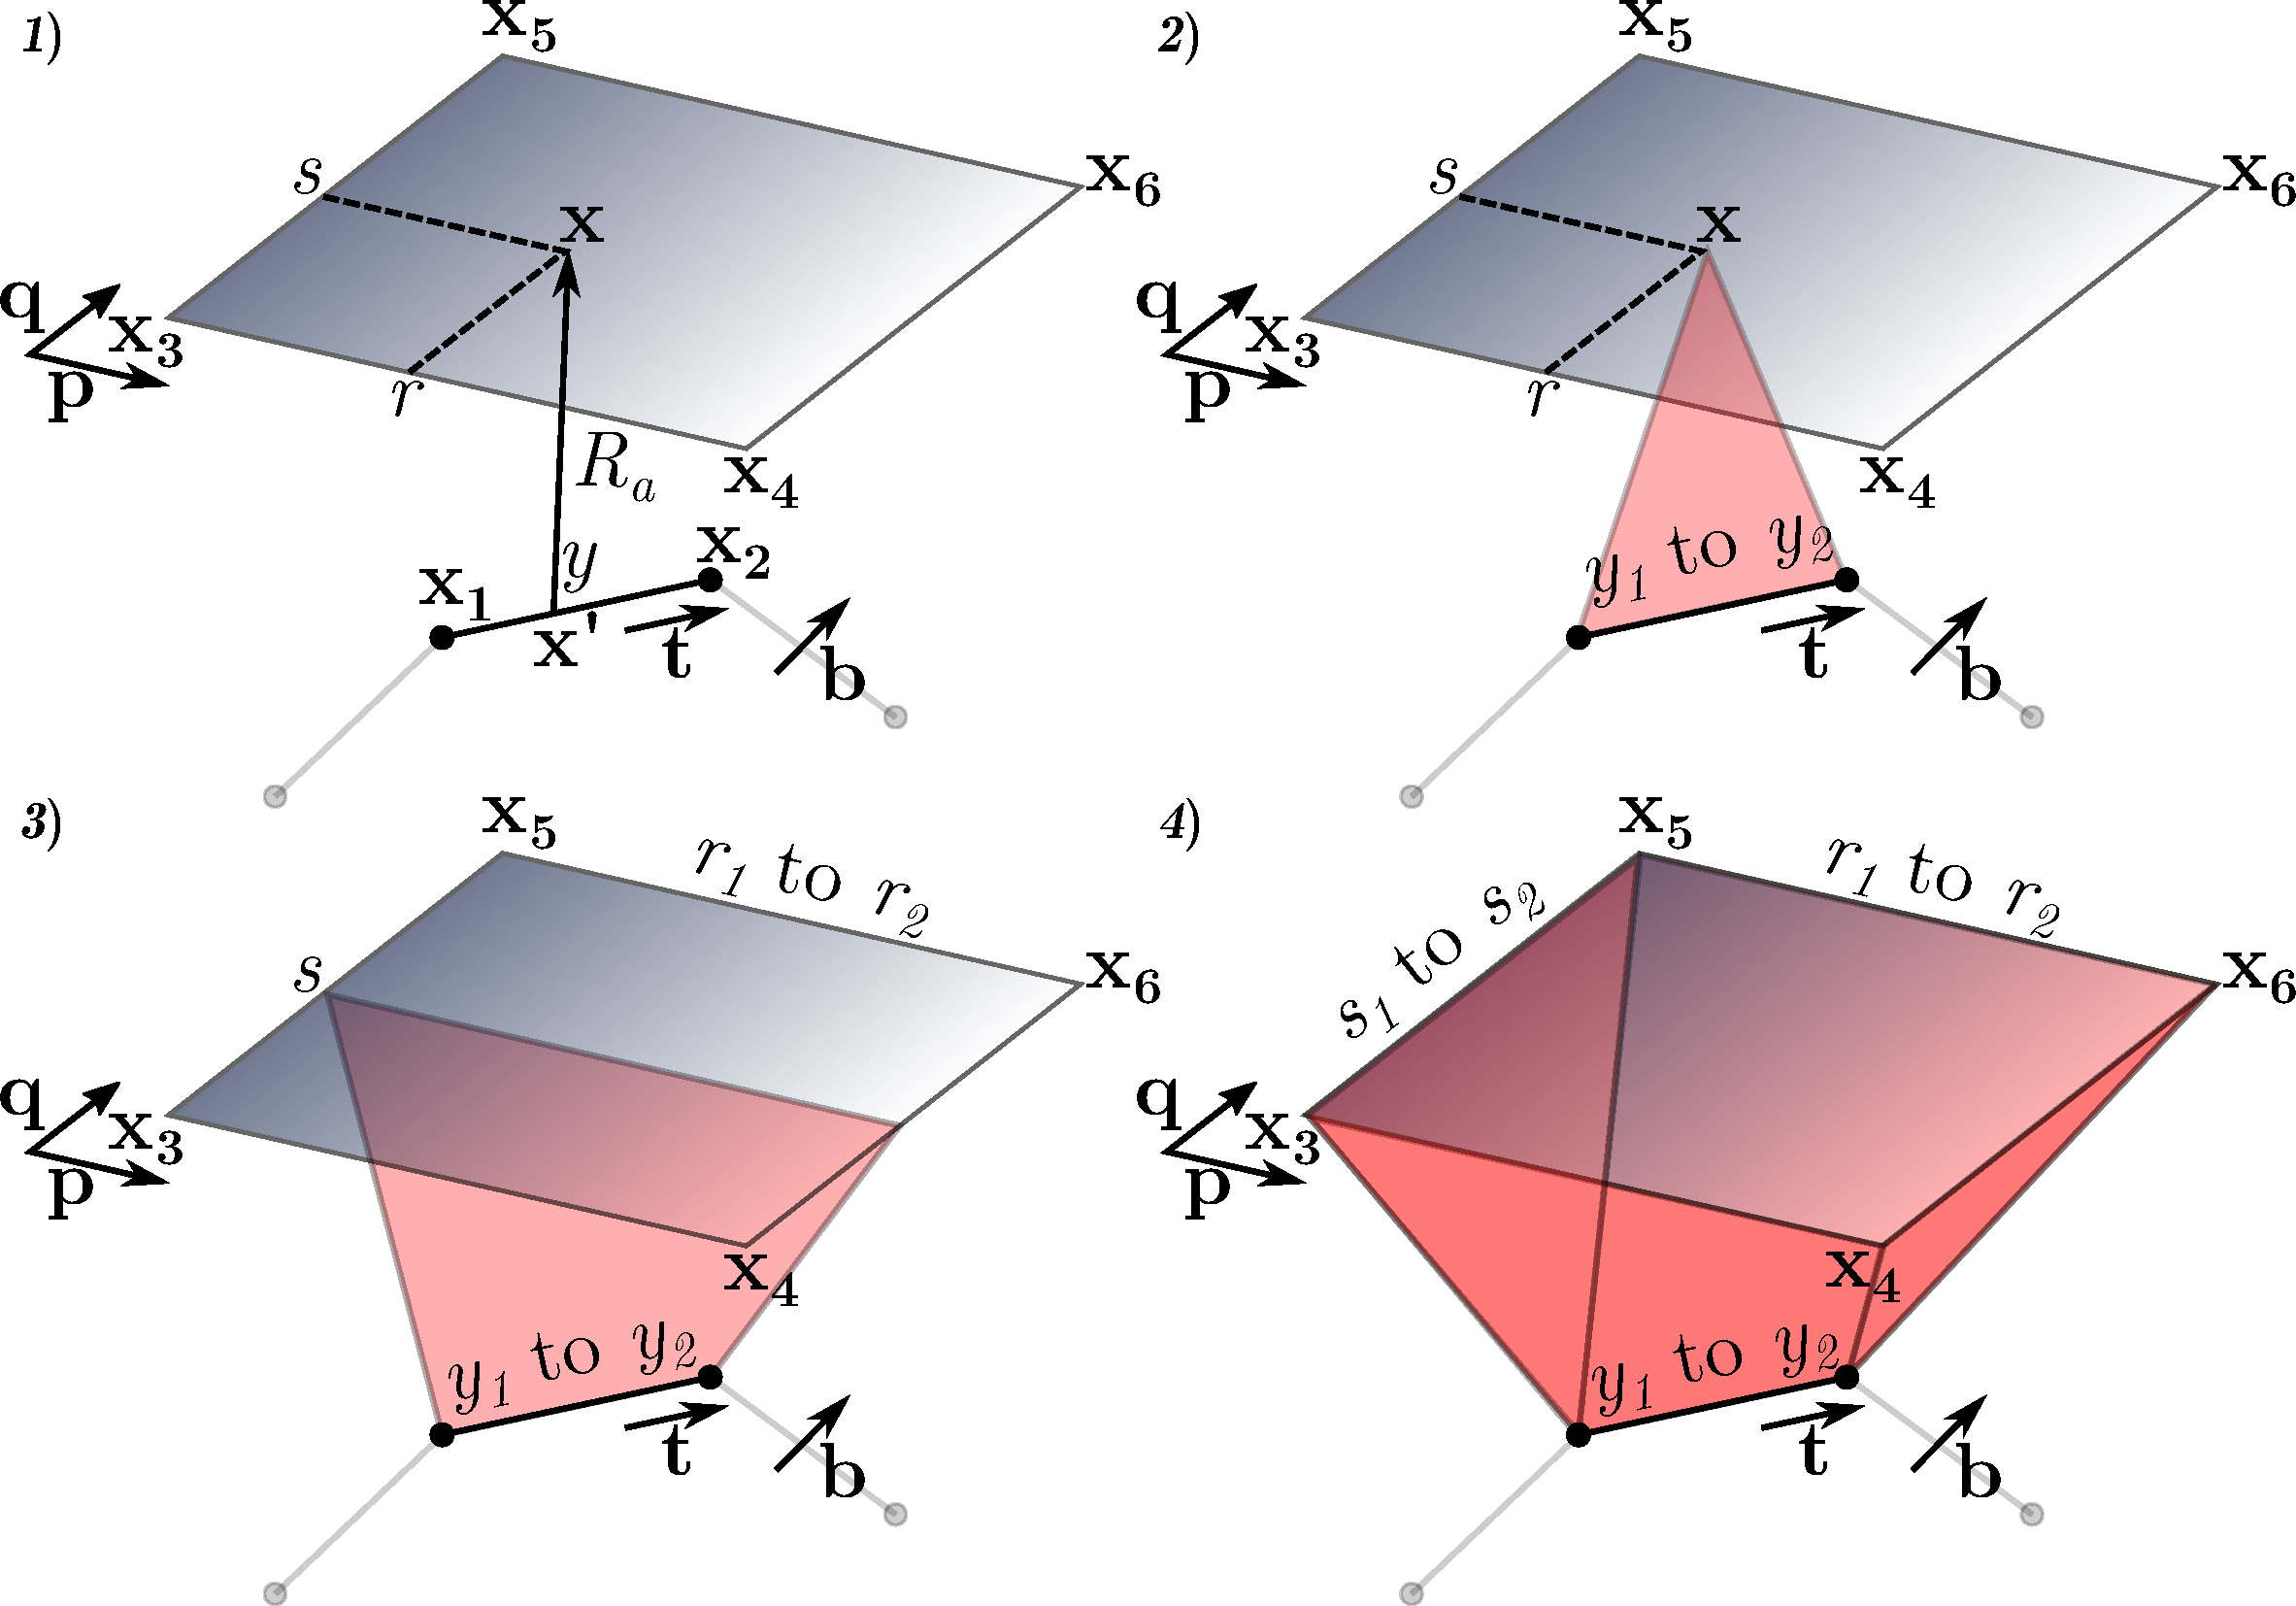
\includegraphics[width=\linewidth]{force_calc_linear_rectangle.pdf}
			\caption[Diagram of the analytical force calculation on linear rectangular surface elements.]{Diagram of the line integral method used to find analytical expressions for the forces exerted by \kwdp{dl} on linear rectangular \kwdp{se} \cite{analytical_integration_of_the_forces_induced_by_dislocations_on_a_surface_element}.
				\textit{1}) For any given point $ \vec{x} $ on the \kwd{se} and any given point $ \vec{x'}$ on the \kwd{dls}, define distance $ R_{a} $.
				\textit{2}) Integrate from $ x_{1} \to x_{2} $ along line direction $ \vec{t} $.
				\textit{3}) Integrate from $ r_{1} \to r_{2} $ along vector $ \vec{p} $.
				\textit{4}) Integrate from $ s_{1} \to s_{2} $ along vector $ \vec{q} $.}
			\label{f:flrs}
		\end{figure}
		\subsection{Resolving Singularities when Dislocation Line Segments are Parallel to Surface Elements}
		\label{ss:par_dln_se}
			%
			\begin{figure}
				\centering
				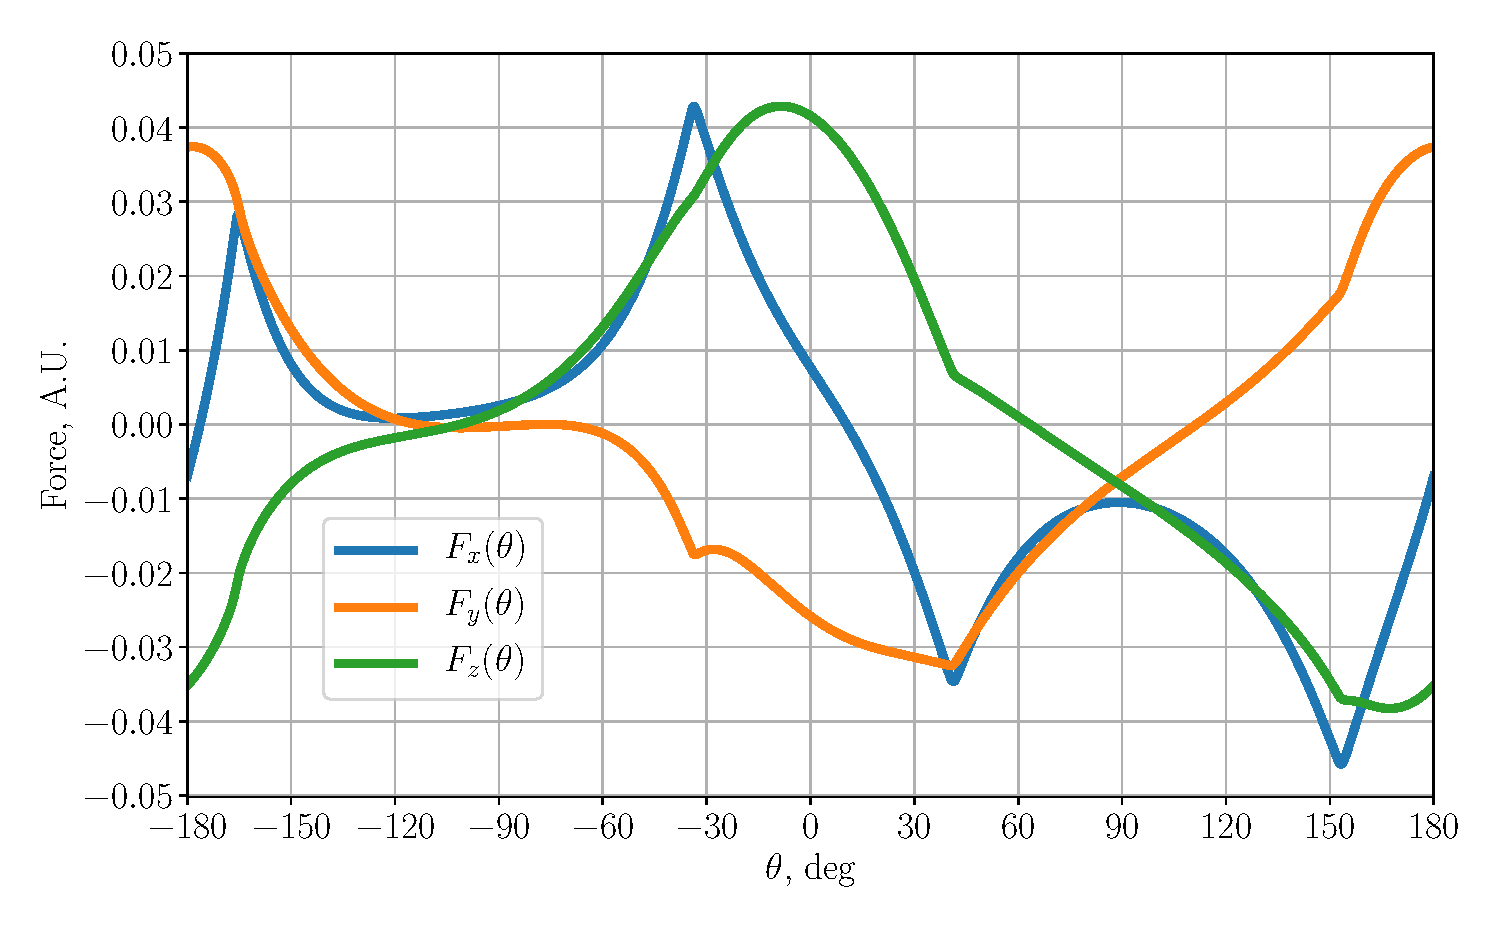
\includegraphics[width=\linewidth]{ftot_rotation_lin_rect.pdf}
				\caption[Avoiding singularities by rotating dislocation line segments.]{Effects of rotating a single \kwd{dls} on the forces exerted by it on a linear rectangular \kwd{se}. The specific values of this function are not known \emph{a priori}, all that is known is that it must be periodic ($ T = 2\pi$) and have finite maximum and minimum values. The singularity is avoided by perturbing the angle $ \theta = 0 \to \theta = \pm \epsilon\,, \epsilon \gtrsim 0 $.}
				\label{f:rflrs}
			\end{figure}
		%
\savearabiccounter